\documentclass[12pt,a4paper]{article}
\usepackage{ctex}
\usepackage{amsmath,amscd,amsbsy,amssymb,latexsym,url,bm,amsthm}
\usepackage{epsfig,graphicx,subfigure}
\usepackage{enumitem,balance}
\usepackage{wrapfig}
\usepackage{mathrsfs,euscript}
\usepackage[usenames]{xcolor}
\usepackage{hyperref}
\usepackage[vlined,ruled,linesnumbered]{algorithm2e}
\usepackage{array}
\usepackage{caption}
\hypersetup{colorlinks=true,linkcolor=black}

\newtheorem{theorem}{Theorem}
\newtheorem{lemma}[theorem]{Lemma}
\newtheorem{proposition}[theorem]{Proposition}
\newtheorem{corollary}[theorem]{Corollary}
\newtheorem{exercise}{Exercise}
\newtheorem*{solution}{Solution}
\newtheorem{definition}{Definition}
\theoremstyle{definition}

\renewcommand{\thefootnote}{\fnsymbol{footnote}}

\newcommand{\postscript}[2]
 {\setlength{\epsfxsize}{#2\hsize}
  \centerline{\epsfbox{#1}}}

\renewcommand{\baselinestretch}{1.0}

\setlength{\oddsidemargin}{-0.365in}
\setlength{\evensidemargin}{-0.365in}
\setlength{\topmargin}{-0.3in}
\setlength{\headheight}{0in}
\setlength{\headsep}{0in}
\setlength{\textheight}{10.1in}
\setlength{\textwidth}{7in}
\makeatletter \renewenvironment{proof}[1][Proof] {\par\pushQED{\qed}\normalfont\topsep6\p@\@plus6\p@\relax\trivlist\item[\hskip\labelsep\bfseries#1\@addpunct{.}]\ignorespaces}{\popQED\endtrivlist\@endpefalse} \makeatother
\makeatletter
\renewenvironment{solution}[1][Solution] {\par\pushQED{\qed}\normalfont\topsep6\p@\@plus6\p@\relax\trivlist\item[\hskip\labelsep\bfseries#1\@addpunct{.}]\ignorespaces}{\popQED\endtrivlist\@endpefalse} \makeatother

\begin{document}
\noindent
\captionsetup[figure]{labelfont={bf},labelformat={default},labelsep=period,name={Fig.}}

%========================================================================
\noindent\framebox[\linewidth]{\shortstack[c]{
\Large{\textbf{Lab11-NP Reduction}}\vspace{1mm}\\
CS214-Algorithm and Complexity, Xiaofeng Gao, Spring 2020.}}
\begin{center}
\footnotesize{\color{red}$*$ If there is any problem, please contact TA Shuodian Yu. }

\footnotesize{\color{blue}$*$ Name:HaotianXue \quad Student ID:518021910506 \quad Email:xavhiart@sjtu.edu.cn}
\end{center}
\begin{enumerate}
	\item What is the ``certificate'' and ``certifier'' for the following problems?
	\begin{enumerate}
		\item \emph{ZERO-ONE INTEGER PROGRAMMING}: Given an integer $m \times n$ matrix $A$ and an integer $m$-vector $b$, is there an integer $n$-vector $x$ with elements in the set $\{0, 1\}$ such that $Ax \leq b$.
		\item \emph{SET PACKING}: Given a finite set $U$, a positive integer $k$ and several subsets $U_1, U_2, \ldots, U_m$ of $U$, is there $k$ or more subsets which are disjoint with each other?
		\item \emph{STEINER TREE IN GRAPHS}: Given a graph $G=(V,E)$, a weight $w(e)\in Z_0^{+}$ for each $e\in E$, a subset $R \subset V$, and a positive integer bound $B$, is there a subtree of $G$ that includes all the vertices of $R$ and such that the sum of the weights of the edges in the subtree is no more than $B$.
	\end{enumerate}
	   
	\begin{solution}
		The certificates and certifiers for the three problems are as follows:
		
		(a)\textbf{ZERO-ONE INTEGER PROGRAMMING}
		  \begin{itemize}
			  \item Certificate: a binary $n$-vector $x$.
			  \item Certifier: Check if $Ax\leq b$.
		  \end{itemize}

		(b)\textbf{SET PACKING}
		\begin{itemize}
			\item Certificate: $k$ subsets $U_{o_i} \in \{U_i|i \in \{1,2,3...,m\}\}(i=1, 2, ..., k)$ 
			\item Certifier: Check if the $k$ subsets are disjoint with each other.
		\end{itemize}

		(c)\textbf{STEINER TREE IN GRAPHS}
		\begin{itemize}
			\item Certificate: Substree $T=(V_t, E_t)$ of $G$ which satisfies: $R \subset V_t$
			\item Certifier: Check if the sum of weights in $T$ is no more than $B$.
		\end{itemize}


    \end{solution}

	\item Algorithm class is a democratic class. Denote class as a finite set $S$ containing every students. Now students decided to raise a student union $S' \subseteq S$ with $|S'|\leq K$ .
	
	As for the members of the union, there are many different opinions. An opinion is a set $S_o\subseteq S$. Note that number of opinions has nothing to do with number of students.
	
	The question is whether there exists such student union $S' \subseteq S$ with $|S'|\leq K$, that $S'$ contains at least one element from each opinion. We call this problem \emph{ELECTION} problem, prove that it is NP-complete.
	
	\begin{solution}
		We can actually reduce the VERTEX-COVER problem to ELECTION problem.
		
		For a VERTEX-COVER instance, we have $G=(V,E)$ and we check if there is a set of vertices that can cover all the edges in $G$. 
	We now regard each edge as an opinion in ELECTION problem, so we have $E=\{e_1, e_2, ..., e_k\}$ functioned to $O = \{S_{o_1}, S_{o_2}, ..., S_{o_k}\}$, where $e_i$ is related to $S_{o_i}$.
	For $e_i = (v_a, v_b)$, we have $S_{o_i} = \{v_a, v_b\}$.  And we can easily prove that $S$ is actually functioned to $V$ respectively, that is, each node in graph is related to one student in the ELECTION problem respectively.

	 Then choose a vertex covering set from $V$ is equivalent to choosing some elements in $S$ which havs common elements with each $S_{o_i}$. That means the choosed set of vertices $S^{'}$ 
	 satisfies the requirements of ELECTION problem.

	 So we can conclude that the VERTEX-COVER is reduced to ELECTION problem. Since the former one is NPC, then we have ELECTION problem is  NPC.
	


    \end{solution}

	\item Not-All-Equal Satisfiability (NAE-SAT) is an extension of SAT where every clause has at least one true literal and at least one false one. NAE-$3$-SAT is the special case where each clause has exactly $3$ literals. Prove that NAE-$3$-SAT is NP-complete. (Hint : reduce $3$-SAT to NAE-$k$-SAT for some $k > 3$ at first)
	\begin{proof}
   
	 We will prove that : $3$-SAT $\leq_{p}$ NAE-$4$-SAT $\leq_{p}$ NAE-$3$-SAT.
	 
	 \begin{itemize}
		 \item $3$-SAT $\leq_{p}$ NAE-$4$-SAT
		  For a clause $C$ = ($x_1 \lor  x_2 \lor x_3$) in one instance of $3$-SAT, we transfer if to $C^{'}=(x^{'}_1 \lor  x^{'}_2 \lor  x^{'}_3 \lor w)$ and we have 
		  $x_i = \sim (x^{'}_i == w)$. So if  $C$ is true then we have at least one $x_i \neq w$, which means $C^{'}$ is satisfied. Otherwise, if $C$ is not true, then all the 
		  $x_i$ is same with $w$, which means the $C^{'}$ is not satisfied.

		 \item NAE-$4$-SAT $\leq_{p}$ NAE-$3$-SAT
		 
		 For an instance in the NAE-$4$-SAT : $C = (x_1 \lor  x_2 \lor x_3 \lor x_4)$ we can break it into $(x_1 \lor x_2 \lor w) \land (\bar{w} \lor x_2 \lor x_4)$.

		 If there are two different elements in $C$, if they are in the same clause in NAE-$3$-SAT, we set $w$ to make the other clause satisfied. Otherwise we just set $w$ to make $w$ and $\bar{w}$ different from 
	 the two different elements in $C$ respectively.

	 If there are no different elements in $C$, it is quite intuitive to see that neither clause in NAE-$3$-SAT can be satisfied.
		\end{itemize}

		So considering $3$-SAT is NPC and the two reductions above, we can conclude that NAE-$3$-SAT is NPC.


    \end{proof}

	\item In the Lab10, we have introduced Minimum Constraint Data Retrieval Problem (MCDR). Prove that MCDR (Version $1$ or $2$) is NP-complete. (Hint : reduce from VERTEX-COVER or $3$-SAT)
	
	\begin{proof}
    We will prove that the VERTEX-COVER problem can be reduced to the MCDR problem.
	 
	First let's define some necessary annotations: 
	
	\begin{itemize}
		\item In the VERTEX-COVER problem we have non-directed graph $G = (V, E)$ and we try to define if we can find a vertex set $S \subset V$ and $|S| \leq k$.
	And $S$ can cover all the edges in $E$.

	   \item We define that the dataset is $D = \{ d_i\}$ and channels are in $C = \{c_i\}$. We have the switches $SW$ and access latency $AL$. And the decision version of $MCDR$ in this case is 
	   defined as : if we can find some way to access all data in $D$, such that $SW < SW_0$ and $LA < LA_0$, where $SW_0, LA_0$ are constant restrictions.

	\end{itemize}

	Then we find one instance for $VERTEX-COVER$as$G = (V,E)$ and $k$. Then we make up the MCDR model like this:

	\begin{itemize}
		\item $C = \{c_1, c_2, ..., c_ {|V|}\} \cup \{ s_1, s_2, ..., s_k\}$, where $c_i$ is related to each node $v_i$ in $V$ and $s_i$ is
		served as the starting points.

		\item The dataset in $MCDR$ are $D = {d_1, d_2, ..., d_{|E|+k}}$, where each data item $d_i(i\in\{1, 2, .., |E|\})$ is related to one edge in $G$. And for each edge $e_{uv}$ we place two data items into  
	channel $c_u$ and $c_v$ just like push data into stacks in any order.
		
	    \item Also for $d_j(j \in \{|E|+1, .., |E|+k\})$ in $D$, it is placed in the first block in $s_j$.
	
		\item We have $2$ empty blocks in each channel for switching, which can be referred to Fig.1. We set the length of all channels to be the same, and the length is noted as $L$, which is equal to $M + 3$ and $M$ is the max degree among all the vertices.
	\end{itemize}
		 
	One example for the model reductions is showed in Fig .1.

	\begin{lemma}
		There is a subset of $V$ with size no more than $k$ which satisfies the vertex-cover if and only if there is a way to fetch data items in $D$ which can satisfiy the restrictions 
		with $(LA, SW) = (kL, 2k-1)$ in $MCDR$ problem.
	\end{lemma}
	
	\begin{proof}
		(1) Firstly, if there is a subset $S$ to cover all the edges in $E$, we only need to choose the corresponding channels $C_{o_1}, C_{o_2}, ..., C_{o_k}$ for those vertices. And we can fetch all the dataitems in these $k$ channels.
		To do this, we start from $s_1$ and go to $C_{o_1}$ and  wait for all the data we want, then we switch from $C_{o_1}$ to $s_2$, then from $s_2$ to $C_{o_2}$, waiting for data in $C_{o_2}$. We repeat like this until all the $k$ channels are tranversed.		
		We can see that in this process, for each channel except the starting channel we have $2$ switches. So the $SW = 2(k-1) + 1 = 2k- 1$ And the time latency can be calculated as $kL$ since we only stay in 
		one channel choosed for one cycle. So we can see that the $MCDR$ restriction is satisfied.

		(2) Then, if we have a satisfied approach to fetch data in $MCDR$ problem. Since we can must fetch data in $s_j(i=1, 2, ..., k)$, then we must have at least $k-1$ switches. The last $k$ switches are used to 
		move between channels , which means we can at moset fetch in $k$ channels. That also means we choose at most $k$ vertices in $G$. So we can get a satisfied vertex set with size on more than $k$ to cover all the edges.
	\end{proof}
	
	According to Lemma 1, we can see that VERTEX-COVER is reduced to MCDR. Since VERTEX-COVER is NPC, we can conclude that the MCDR is NPC.
	

	\begin{figure}

    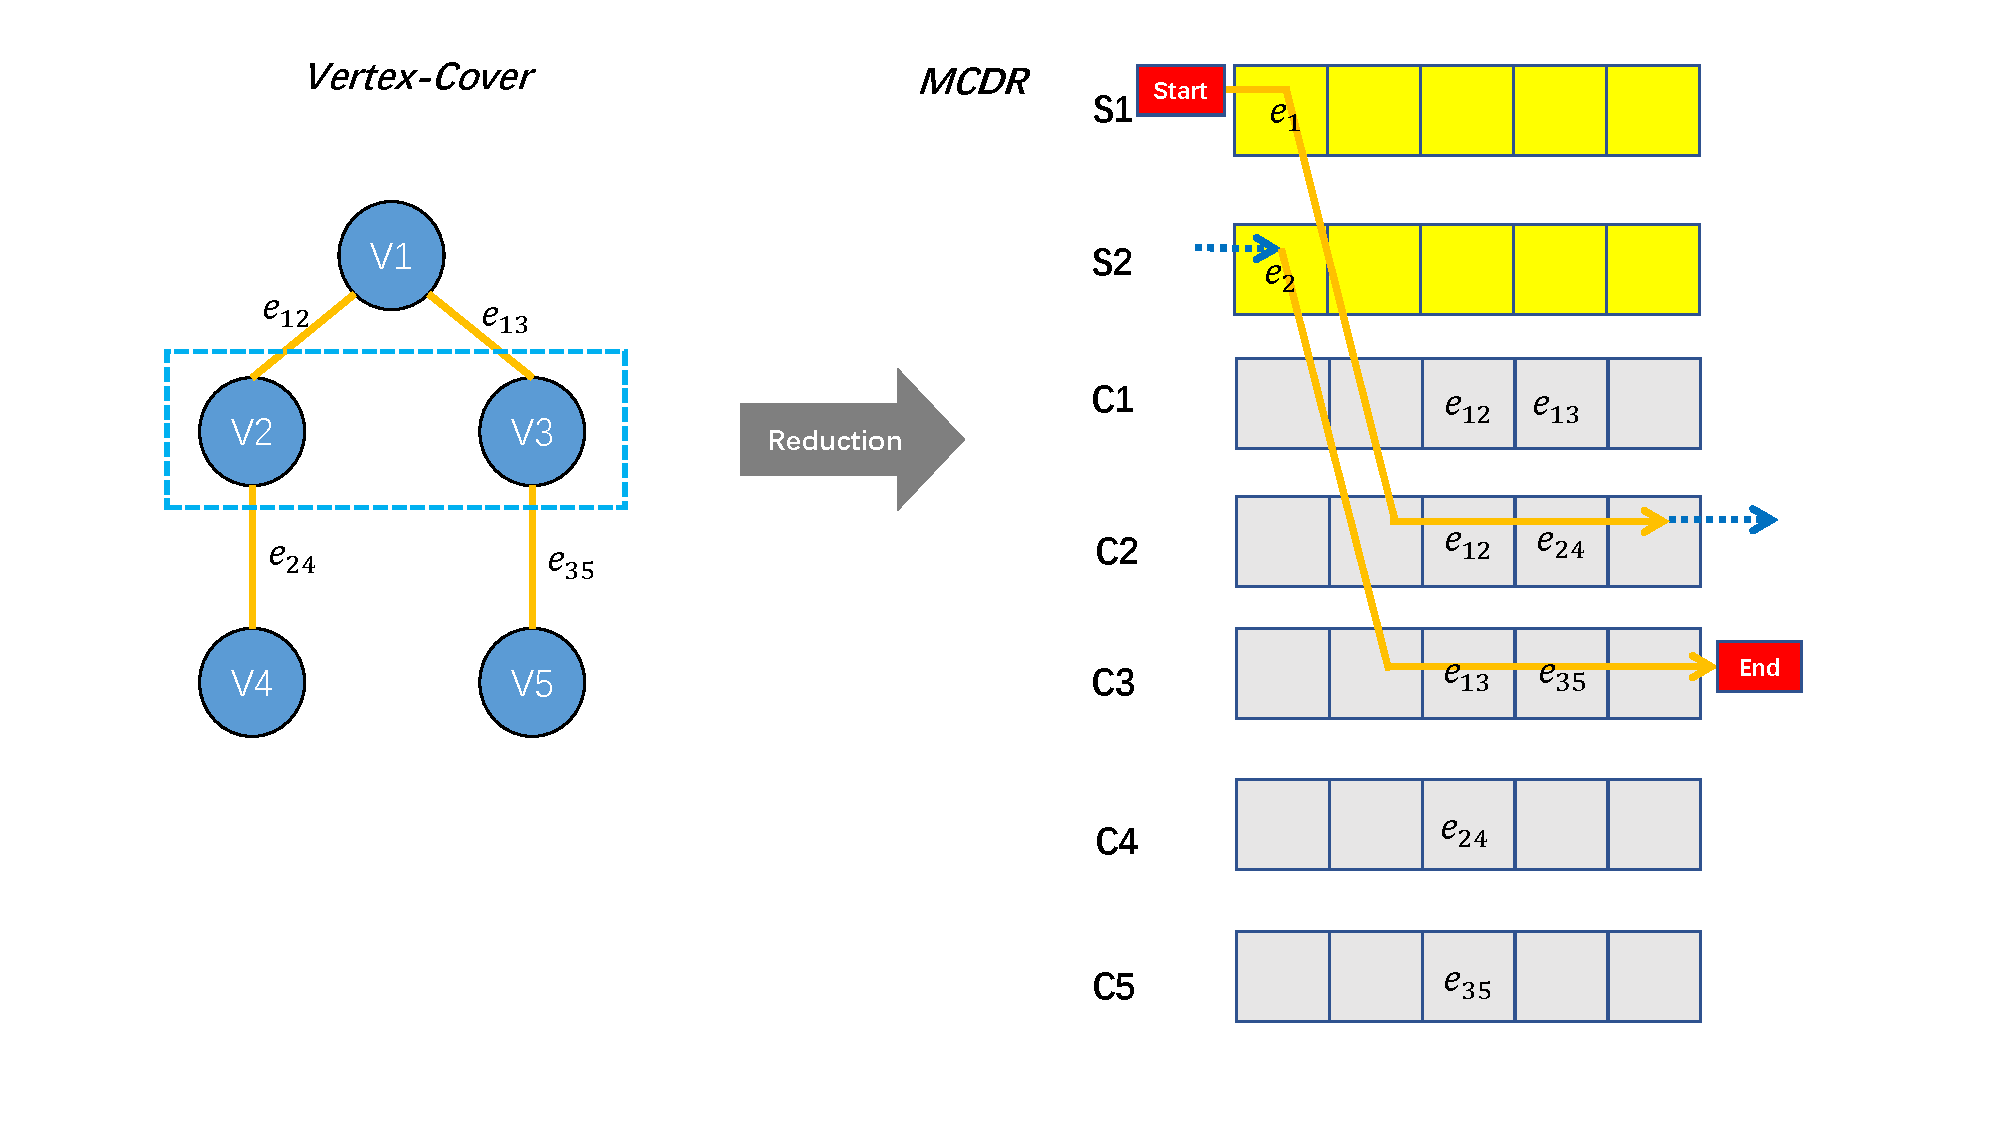
\includegraphics[scale=0.6]{MCDR.pdf}
    \caption{Reduction from VERTEX-COVER to MCDR}

	\end{figure}
\end{proof}
\end{enumerate}

\textbf{Remark:} Please include your .pdf, .tex files for uploading with standard file names.




%========================================================================
\end{document}
